\chapter{Introduction}

\section{Nuclear Power} % Complete

In the summer of 1956, the world's first commercial nuclear power plant was connected to the grid in the north of England. This marked a significant departure from previous forms of commercial energy production, which relied on relatively low energy density sources such as combustion of coal, oil and gas. Before this, the closest anyone had come to utilising nuclear energy commercially was through geothermal power, where the thermal energy input is partly due to radiogenic heat from unstable isotopes in the Earth's mantle \cite{gando2011partial}. 
%which relied on the chemical reactions of coal oil and gas
%Combustion is a chemical process, where energy differences between reactants and products are exploited via electron exchange. Nuclear energy however, exploits the energy difference between nuclei. Both rely on the conversion of mass into energy, however, the amount of energy that can be extracted varies by several orders of magnitude
Combustion is a chemical process whereby energy differences between reactants and products are exploited via electron exchange. Nuclear energy however, exploits the energy difference between nuclei. Both rely on the conversion of mass into energy, however, the amount of energy that can be extracted from the nucleus is several orders of magnitude greater.
%Combustion is a chemical process, and its use in commercial energy production is fundamentally about exploiting the free energy difference when electrons are exchanged between some reactants to produce some products. Nuclear energy, however, is about the direct conversion of mass into energy. The difference between the two is staggering.

Consider methane, with an enthalpy of combustion of −887.2 kJ/mol \cite{thornton1917xv}. This is the equivalent of 9.14 eV per particle. By comparison, the total energy release from fission of one uranium-235 nucleus is at least $1.65 \times 10^{8}$ eV, as shown in Figure \ref{figure:fissionenergy}.

Combustion-based power as a technology has matured over hundreds of years, with modern optimisations only looking to offer fractional percent gains in efficiency. By comparison, nuclear power technology is far from mature, with large improvements yet to be realised. One such feature is load-following, an enormously useful feature for a power plant which is currently unavailable in nuclear reactors. The biggest obstacle to achieving load-following in nuclear reactors is the issue of pellet-cladding interaction (PCI), which is the basis of the work in this thesis.

\begin{figure}[htp]
\centering
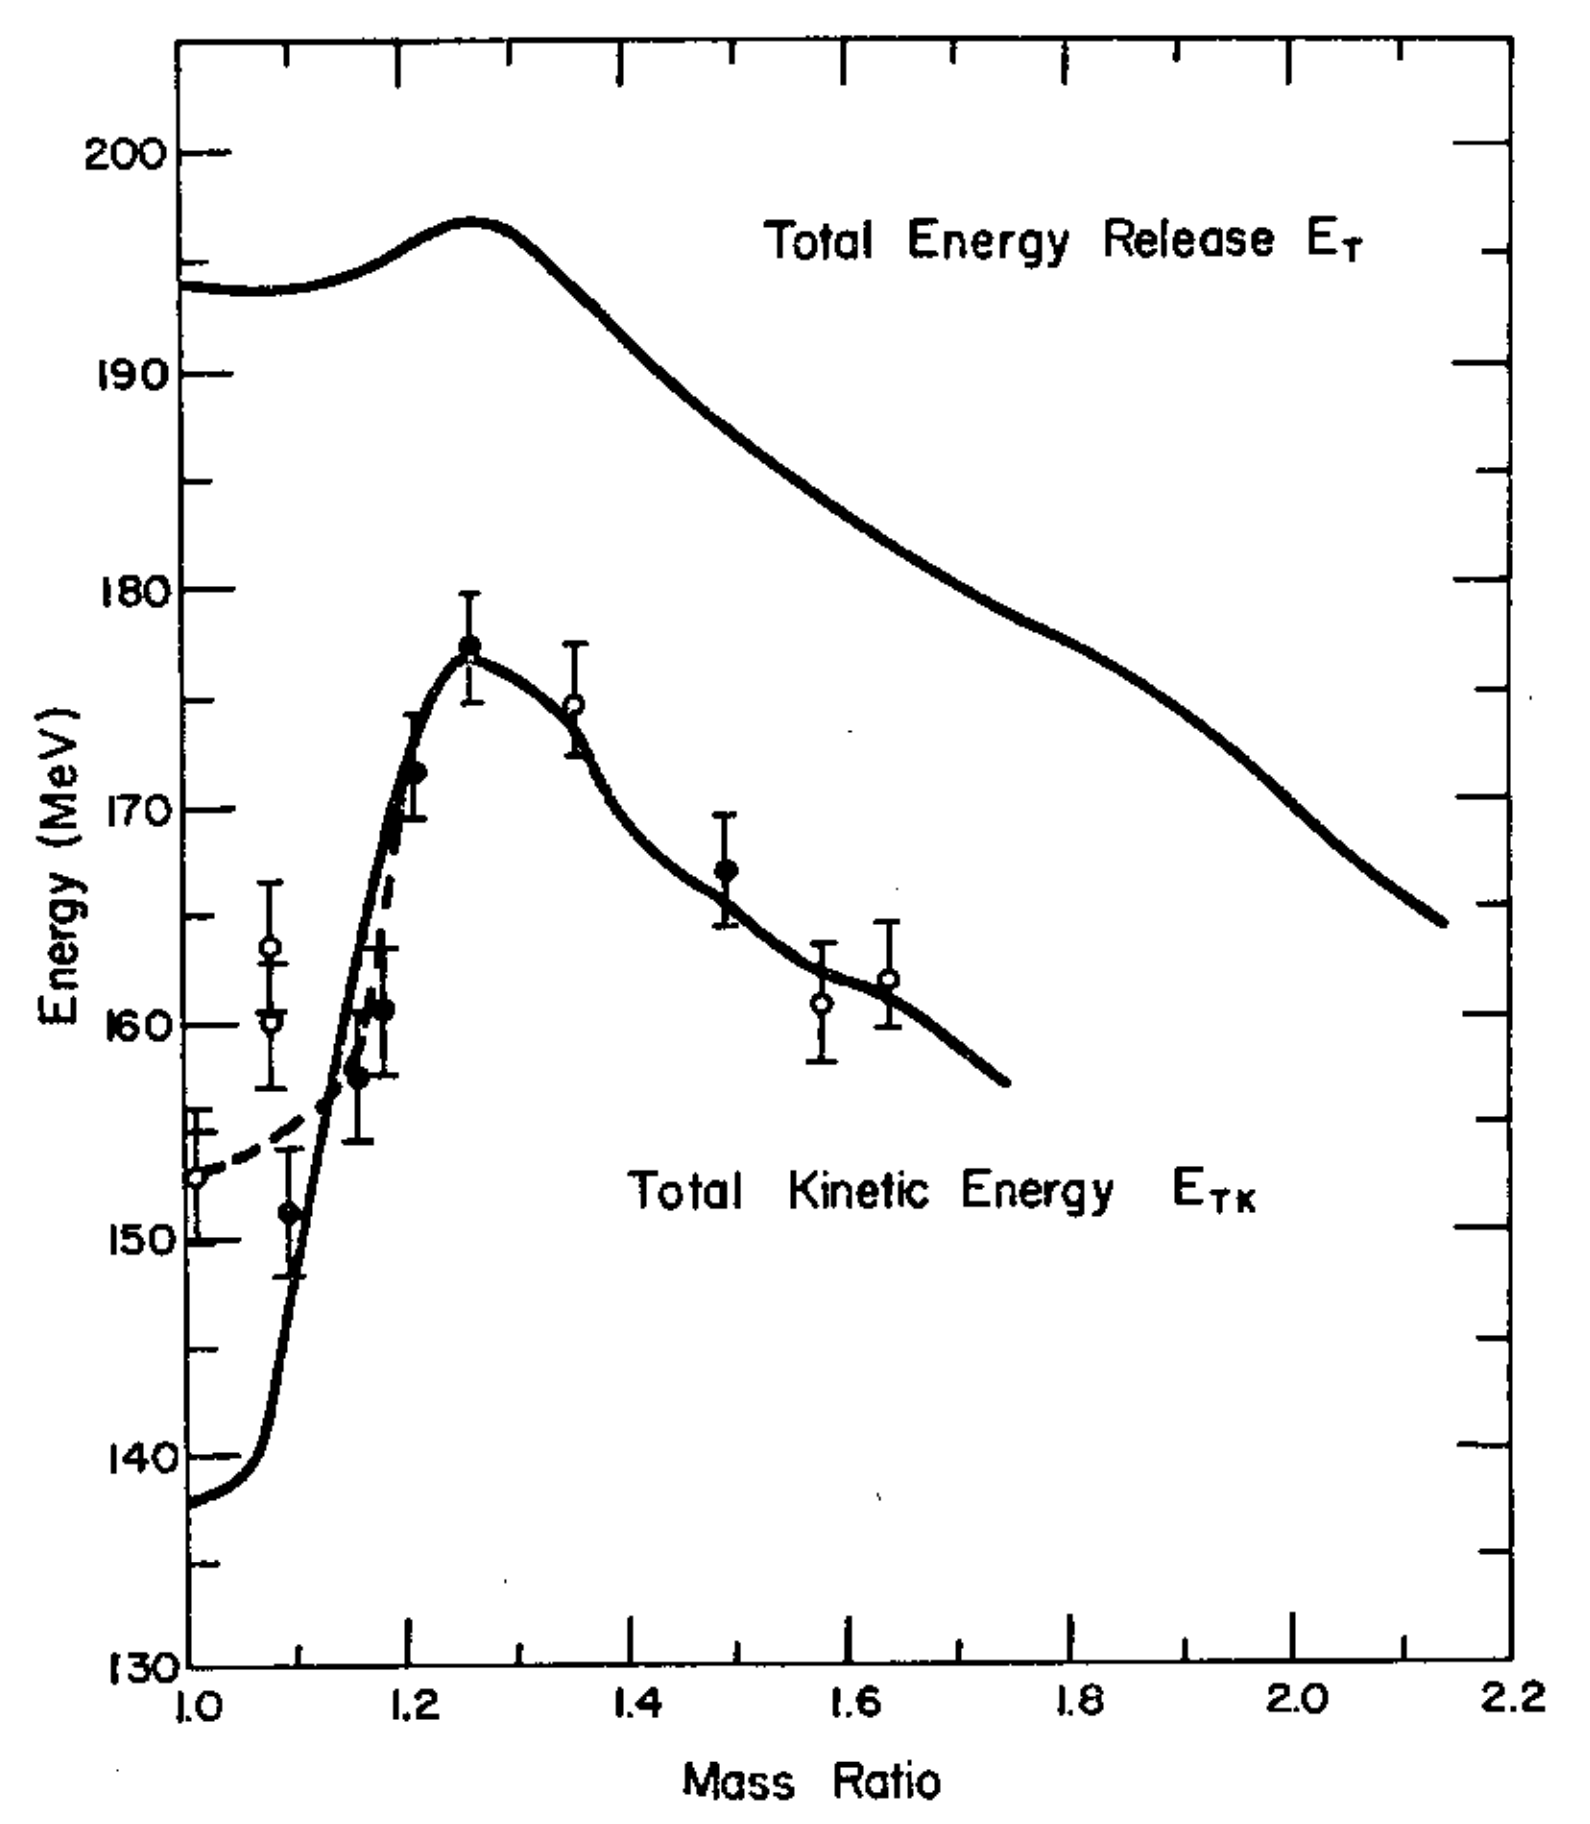
\includegraphics[height=13cm]{images/fission_energy_total.png}
\caption[Energy from thermal fission of U-235 as a function of mass ratios of child nuclei. Total energy release includes contributions from gamma rays and subsequent radioactive decays.]{Energy from thermal fission of U-235 as a function of mass ratios of child nuclei. Total energy release includes contributions from gamma rays and subsequent radioactive decays. Taken from \cite{aras1965ranges}.}
\label{figure:fissionenergy}
\end{figure}

\subsection{Fission} % Complete

Commercial nuclear power plants extract energy through the process of fission, where a large nucleus is split into smaller nuclei. While it is also possible to extract energy from certain nuclei by the process of fusing them into larger ones, no fusion reactor currently exists which achieves a net positive energy output. At a fundamental level, both of these processes rely upon mass-energy equivalence. The relationship between mass and energy is shown using Einstein's famous equation:

\begin{equation}
\label{emc2}
    E = mc^{2}
\end{equation}

where $E$ is the energy of the system, $m$ is the mass and $c$ is the speed of light. Using this equation we can analyse a typical fission reaction:

\begin{equation}
    U^{235}_{92} + n^{1}_{0} \longrightarrow I^{132}_{53} + Y^{101}_{39} + 3n^{1}_{0}
\label{eqn:fission} 
\end{equation}

While the number of protons and neutrons are conserved throughout the reaction, a quick calculation will show that there is actually less mass in the products than the reactants by approximately 0.188 amu (3.127$\times 10^{-28}$ kg). This missing mass, known as the \emph{mass defect}, is converted to energy ($\sim$175 MeV). In this way, the total mass-energy of the system is conserved. 

This change in mass arises due to the phenomenon of \emph{binding energy}. In order for two or more nucleons to be thermodynamically stable when bound together, the total free energy of the bound configuration must be less than the sum of constituent nucleon free energies. Much like with energy stored in a chemical bond, the binding energy represents the energy required to separate the nucleus into individual protons and neutrons. 

Larger nuclei will generally have a greater total binding energy value compared to smaller nuclei, but the mass defect per nucleon will not necessarily be greater in a larger nucleus. It is therefore useful to normalise the binding energy by the mass number. Different isotopes have different binding energies, and any nuclear reaction which increases the binding energy per nucleon will be exothermic, whether by fission or fusion. Figure \ref{figure:bindingenergy} shows a plot of binding energy per nucleon against mass number with the relevant isotopes from Equation \ref{eqn:fission}. 

%235.0439299 + 1.008664 (236.0525939) -> 131.907997 + 100.93031 + 3.025992 (235.864299)




\begin{figure}[htp]
\centering
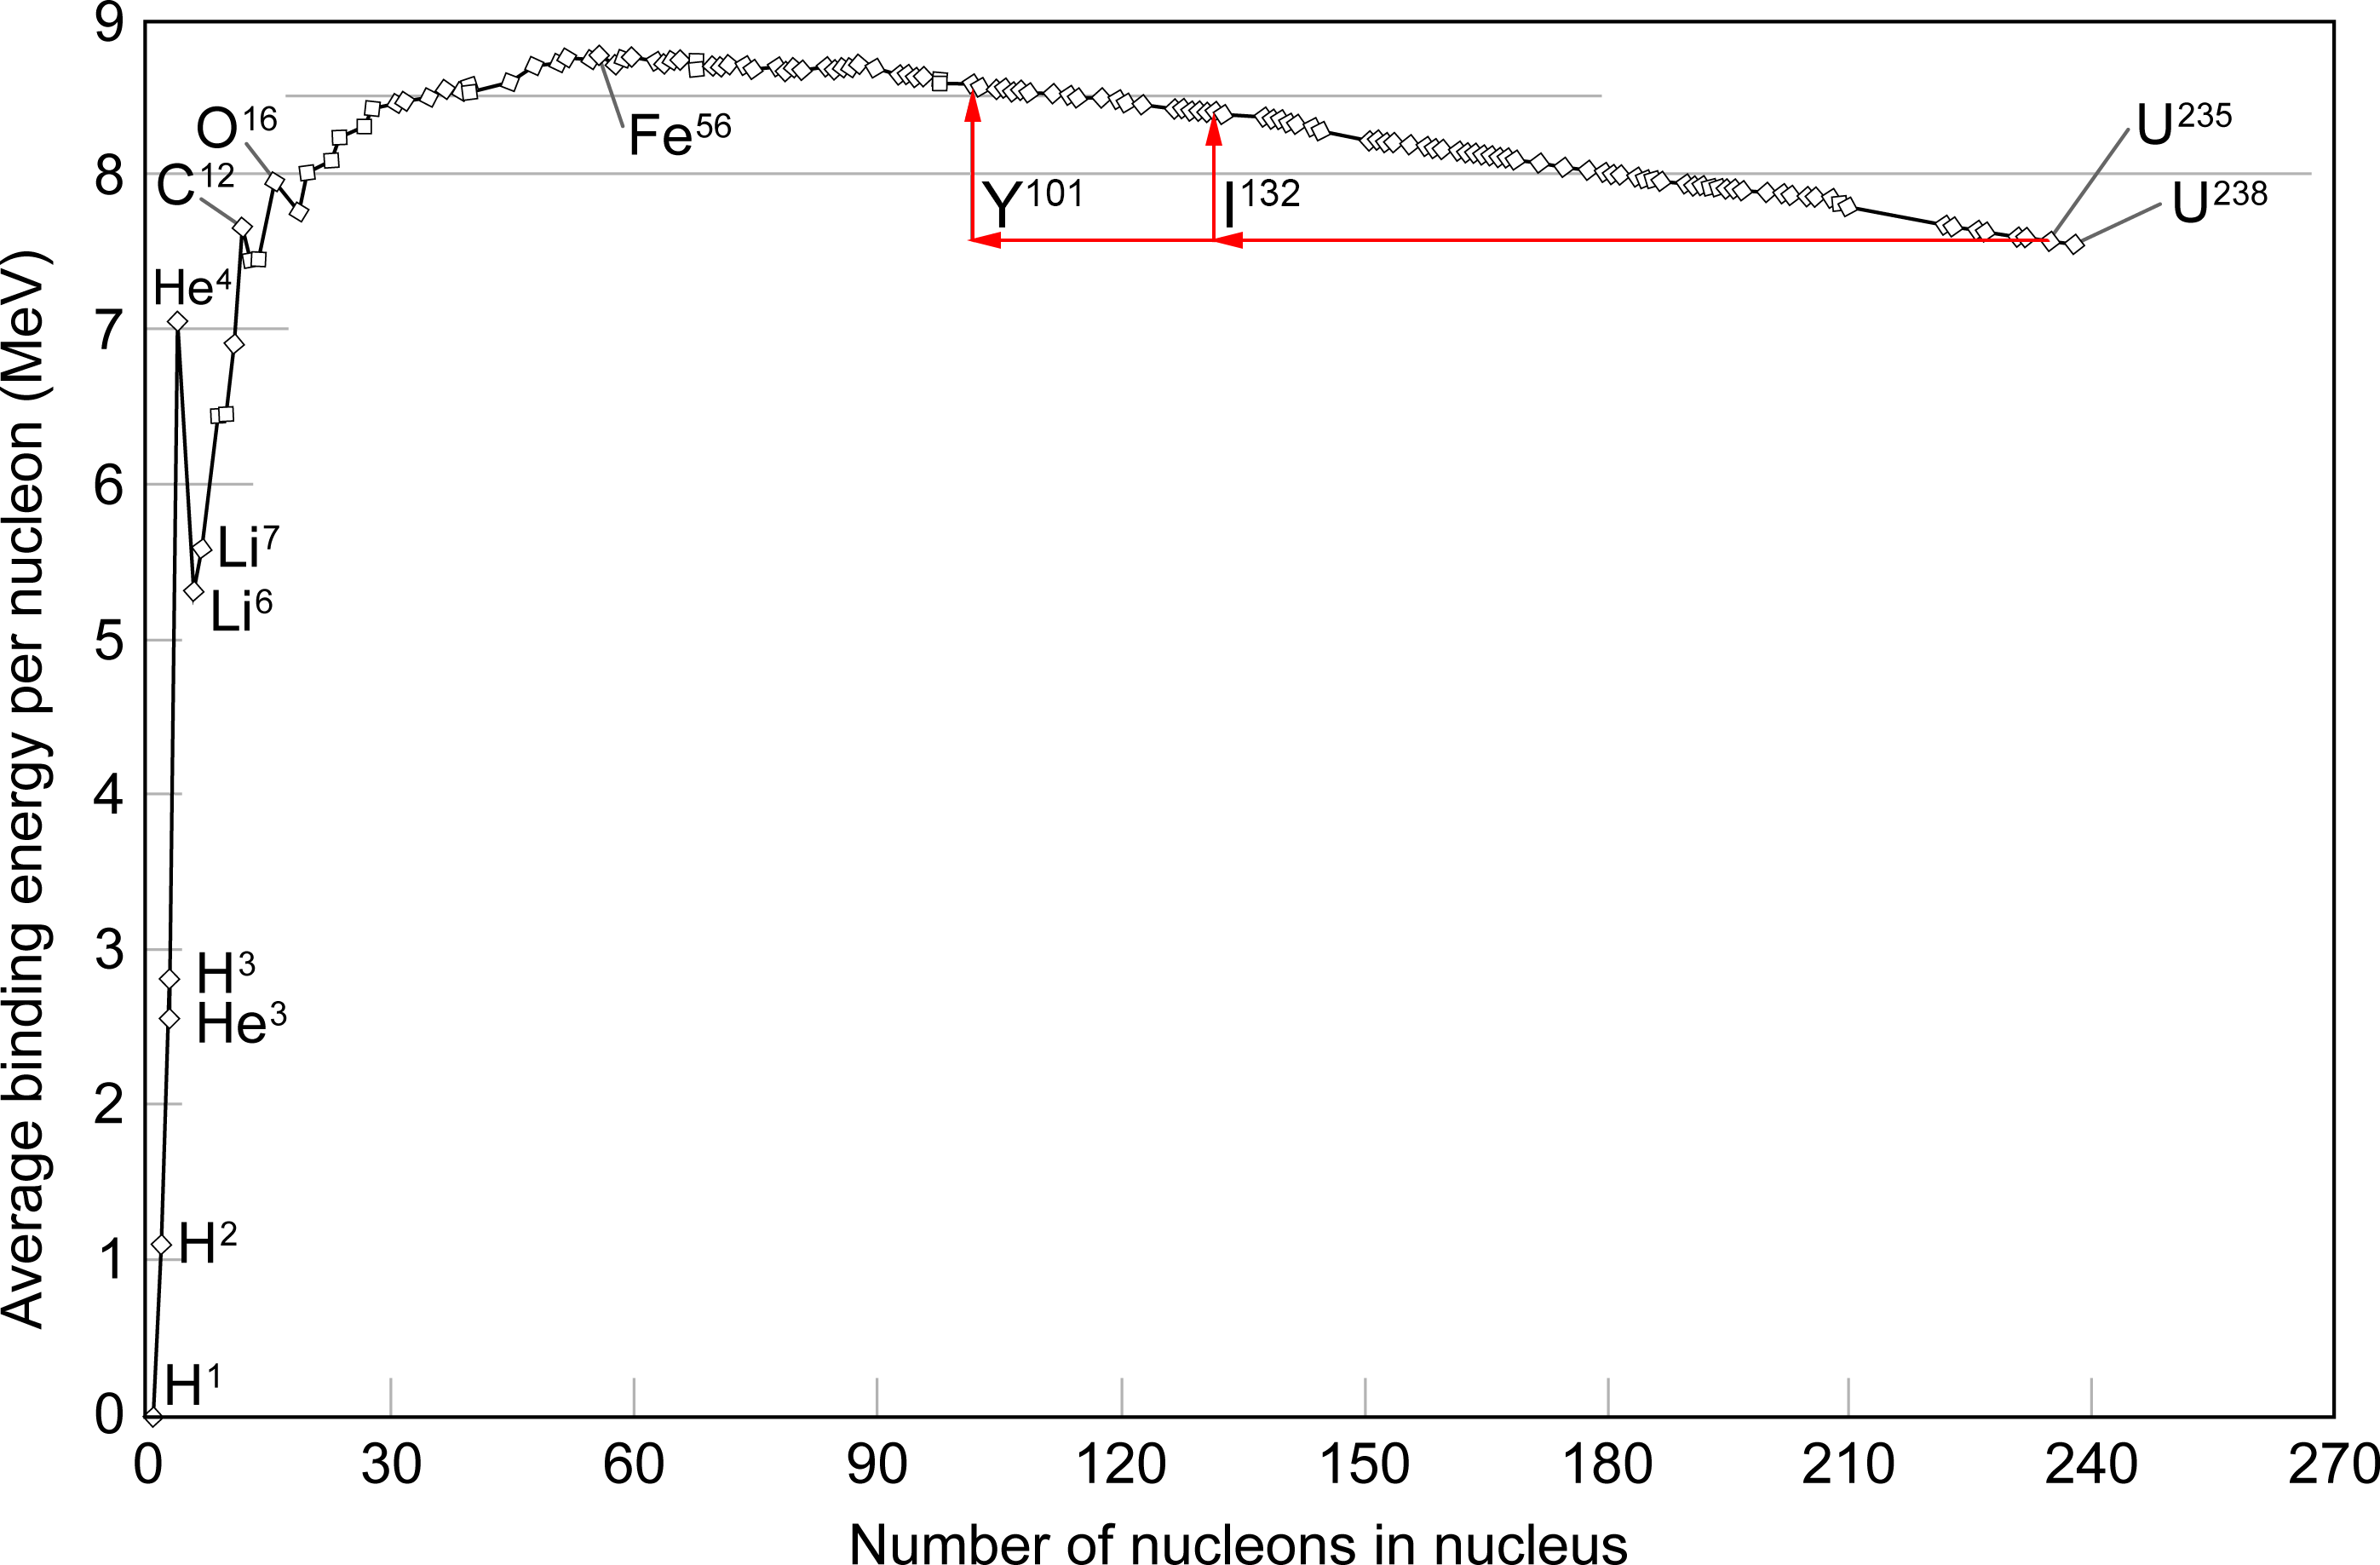
\includegraphics[width=14cm]{images/Binding_energy_curve.png}
\caption[Plot binding energy per nucleon against mass number. Arrows indicate the reaction shown in equation \ref{eqn:fission}.]{Plot binding energy per nucleon against mass number. Arrows indicate the reaction shown in equation \ref{eqn:fission}. Adapted from \cite{Fastfission}.}
\label{figure:bindingenergy}
\end{figure}


\subsection{Reactor design} % Complete

Commercial nuclear reactors are large boilers in a Rankine cycle, designed to maximise heat transfer to a working fluid. All nuclear plants use steam turbines on the generation side, though the reactor coolant may be another fluid in a separate loop, such as carbon dioxide in gas-cooled reactors (GCRs), or even in a separate water loop such as in pressurised water reactors (PWRs) and CANDU. 

The most prevalent reactor type is the PWR, followed by the boiling water reactor (BWR). There are several other reactor types used around the world (enumerated in Figure \ref{figure:world_reactors}). The work in this thesis is focused on zirconium-based claddings which are used worldwide in all commercial reactors except GCRs and sodium-cooled fast reactors. In total, zirconium fuel cladding is used in over 95\% of all nuclear reactor fuel pins, and so improvements in these cladding materials have an effect across the entire industry.

\begin{figure}[htp] % Reactors in the world
\centering
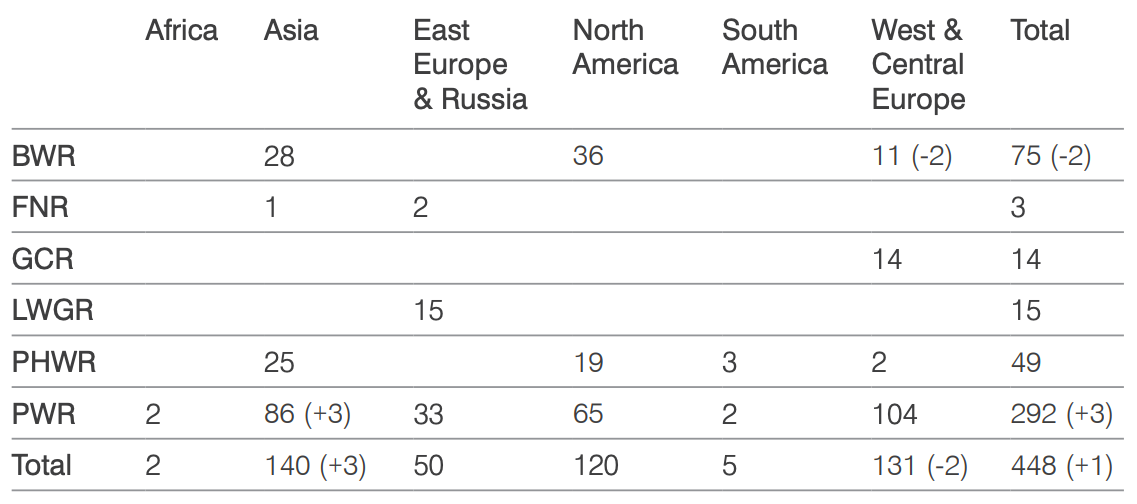
\includegraphics[width=15cm]{images/WNA_report2018.png}
\caption[Type and number of different reactors operational worldwide as of the end of 2017.]{Type and number of different reactors operational worldwide as of the end of 2017. Taken from \cite{WNAreport2018}.}
\label{figure:world_reactors}
\end{figure}

The fission of uranium takes place inside a steel reactor pressure vessel (RPV) which holds the fuel pins and control rods. The working fluid in a nuclear reactor is typically under high pressure, with PWR RPV operating pressures between 150 and 160 bar, while BWRs operate at lower pressures of around 70 bar \cite{kok2016nuclear, Server2010, Durmayaz2001}. The pressure of the coolant acts on the fuel cladding, generating radial and hoop stresses which influence crack formation. 

The operating temperature of the coolant in a typical PWR is approximately 600 K. This is a low temperature relative to the melting points of zirconium (2128 K) and zirconia (2988 K). This temperature together with the high pressure is chosen in order to keep the coolant in the liquid phase for safety reasons, though this limits the thermodynamic efficiency of the plant. The highest temperature in a reactor will occur in the nuclear fuel, with PWR fuel pellets reaching centreline temperatures of up to 1673 K \cite{beyer1998review}.

For both PWRs and BWRs, the coolant is typically light water (as opposed to heavy water, D$_{2}$O). Water is used because it has many useful properties. It is cheap, plentiful, has a high heat capacity (compared to the gaseous coolant in gas cooled reactors), has low activation in a free neutron environment and also serves as a good radiation shield. 

In additional to its function as a coolant, water also acts as a neutron moderator, slowing down high-energy neutrons from fission events and nuclear decay processes. Moderation of neutrons is an important step in the nuclear reactor because slow thermal neutrons (i.e. neutrons at thermal equilibrium with the coolant) are significantly more likely to fission uranium nuclei than fast neutrons. Fast neutrons will typically escape from the fuel pin after they are generated, dispense most of their energy in the coolant via scattering with H and O nuclei, and then some will end up re-entering the fuel, where they will most likely fission a U$_{235}$ nucleus near the outer edge of the fuel pellet. Neutrons which don't end up fissioning fuel will either be absorbed parasitically by other nuclei (likely in the control rods), escape from the reactor entirely (neutron leakage), or decay into protons (free neutrons have a half-life of 15 minutes).


\subsection{Fuel pins and cladding} \label{ss_fuelpin}

Fuel assemblies in nuclear reactors are bundles of fuel pins. In most commercial reactors, these fuel pins are comprised of a zirconium-based cladding which is filled with UO$_{2}$ fuel pellets, each of which are approximately 1 cm$^{3}$ in volume. Once loaded with fuel pellets, the fuel pins are capped and filled with inert helium gas, pressurised to between 2 and 25 atm to improve heat transfer from the fuel pellets to the coolant as well as delaying inward creep deformation of the cladding due to the high coolant pressure \cite{King1980}. 

In the early stages of a fuel pin's life, there is a small gap between the fuel pellet and the cladding, known as the pellet-cladding gas gap. This gas gap slowly closes with increasing burn-up due to swelling of the fuel pellets and inward creep deformation of the cladding. The pellet-cladding system is shown using a view of the cross section of a PWR fuel pin in Figure \ref{figure:gas_gap}. The cladding internal oxide layer covers the entire internal circumference of the cladding and is the first barrier to corrosive species. 

\begin{figure}[htp]
\centering
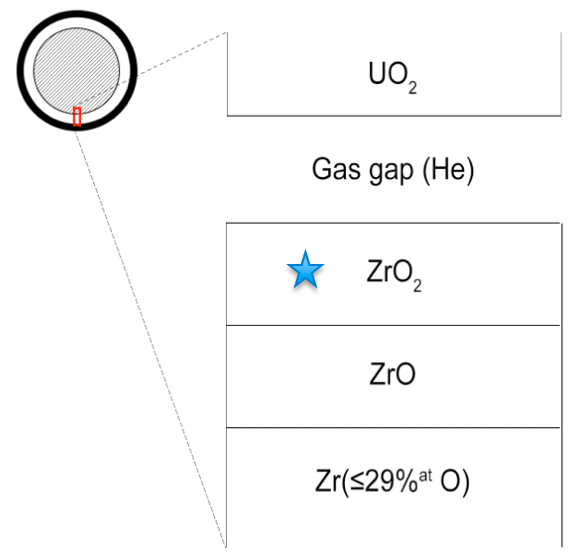
\includegraphics[width=10cm]{images/gas_gap.png}
\caption{Schematic view of a single PWR fuel pin cross section with an expanded view of the pellet-gap-cladding system.}
\label{figure:gas_gap}
\end{figure}


\subsection{Effects of radiation on materials} 

While ionising radiation is always present in the environment as background radiation, the intensity of radiation in a nuclear reactor is so great that it presents significant engineering challenges because of how it affects different materials.

Radiation hardening (also known as radiation embrittlement) is a phenomenon which affects most materials subjected to ionising radiation. It is characterised by a loss of plasticity caused by radiation damage over time, leading to an increased risk of cracks and failure of components. While zirconium is a very useful nuclear material due to it's neutron transparency, it is still susceptible to this type of damage \cite{Wisner1998}. Beyond certain levels of radiation damage, phase changes may also occur. %In \zirconia\ however,  

Amorphisation is another effect of radiation damage. This is characterised by a loss of long-range order of atoms in a crystal. This typically occurs beyond a certain threshold of radiation damage depending on the material, called the critical amorphisation dose. Amorphisation is problematic because the loss of a defined crystal structure results in both a reduction in structural stability (amorphous materials have a higher Gibbs free energy than their crystalline counterparts) and causes swelling of the material \cite{Einfal2013}. In the literature, there is evidence of amorphisation in cubic stabilised \zirconia\ when bombarded with Cs$^{+}$ ions up to a fluence of $1 \times 10^{21}$ ions m$^{-2}$ \cite{amorphization2000wang}. However, no amorphisation is seen at an Xe$^{2+}$ fluence of $2 \times 10^{21}$ ions m$^{-2}$, or an I$^{+}$ fluence of $5 \times 10^{19}$ ions m$^{-2}$ \cite{sickafus1999radiation}.

One material phenomenon exclusive to nuclear reactor environments is neutron activation. The high free neutron environment leads to neutron capture in various nuclei within the reactor, including those of the fuel assemblies, coolant and RPV. There are many possible (n, x) reactions that may occur in materials experiencing a neutron flux, but of particular concern is transmutation of nuclei following a nuclear capture event. When a stable nucleus captures a neutron and becomes unstable, the nucleus may then emit particles to reduce it's free energy, altering it's atomic number in the process. This new element will have different chemical properties compared to the parent nucleus by virtue of a different electronic structure. This will change the elemental composition of a material, typically in an unfavourable way with dopants that negatively affect some desired material property. The extremely large number of nuclei relative to neutron flux means that this effect is small, though over time this becomes more significant due to accumulation of these dopant elements.

In high-radiation environments, it is also possible for some molecules to be split by gamma photons above certain energies through the process of radiolysis. Corrosive fission products such as iodine will be present inside the fuel pin, but present in the form of CsI which is not highly corrosive. Radiolysis however, decomposes CsI into Cs and I$_{2}$ vapour which can diffuse towards the cladding and promote cracking \cite{Konashi1983}.

\subsection{Fission products, their distribution and decay chains}

Nuclei which can undergo fission will produce child nuclei (fission products) with specific characteristics. Firstly, these nuclei will almost always be neutron-rich, as compared to their stable isotopes. This is the result of the higher neutron to proton (N/Z) ratios of larger nuclei. Figure \ref{figure:NZcurve} shows how the nuclei of abundant isotopes start with N/Z ratios of around 1 for small elements (e.g. \ch{He_{2}^{4}}, \ch{C_{6}^{12}}, \ch{O_{8}^{16}}), whereas larger elements will have isotopes with N/Z ratios approaching 1.6 (e.g. \ch{Pb_{82}^{208}}, \ch{Th_{90}^{232}}, \ch{U_{92}^{238}}). 

Fissionable nuclei are typically very large and when fission occurs, the child nuclei will inevitably inherit a high N/Z ratio. These neutron-rich nuclei will generally decay by $\beta-$ particle emission to reduce their N/Z ratio and increase stability. One decay event is usually not enough to achieve a stable nucleus, so several decays as part of a decay chain are expected (Equations \ref{eqn:te_decay} and \ref{eqn:i_decay}).

{\setstretch{1.3}
\begin{equation}
Te_{134}^{52} \xrightarrow[]{\beta-} I_{134}^{53}+ e^{-} + \overline{\nu}_{e}
\label{eqn:te_decay}
\end{equation}

\begin{equation}
I_{134}^{53} \xrightarrow[]{\beta-} Xe_{134}^{54} + e^{-} + \overline{\nu}_{e}
\label{eqn:i_decay}
\end{equation}
}

\begin{figure}[ht]
\centering
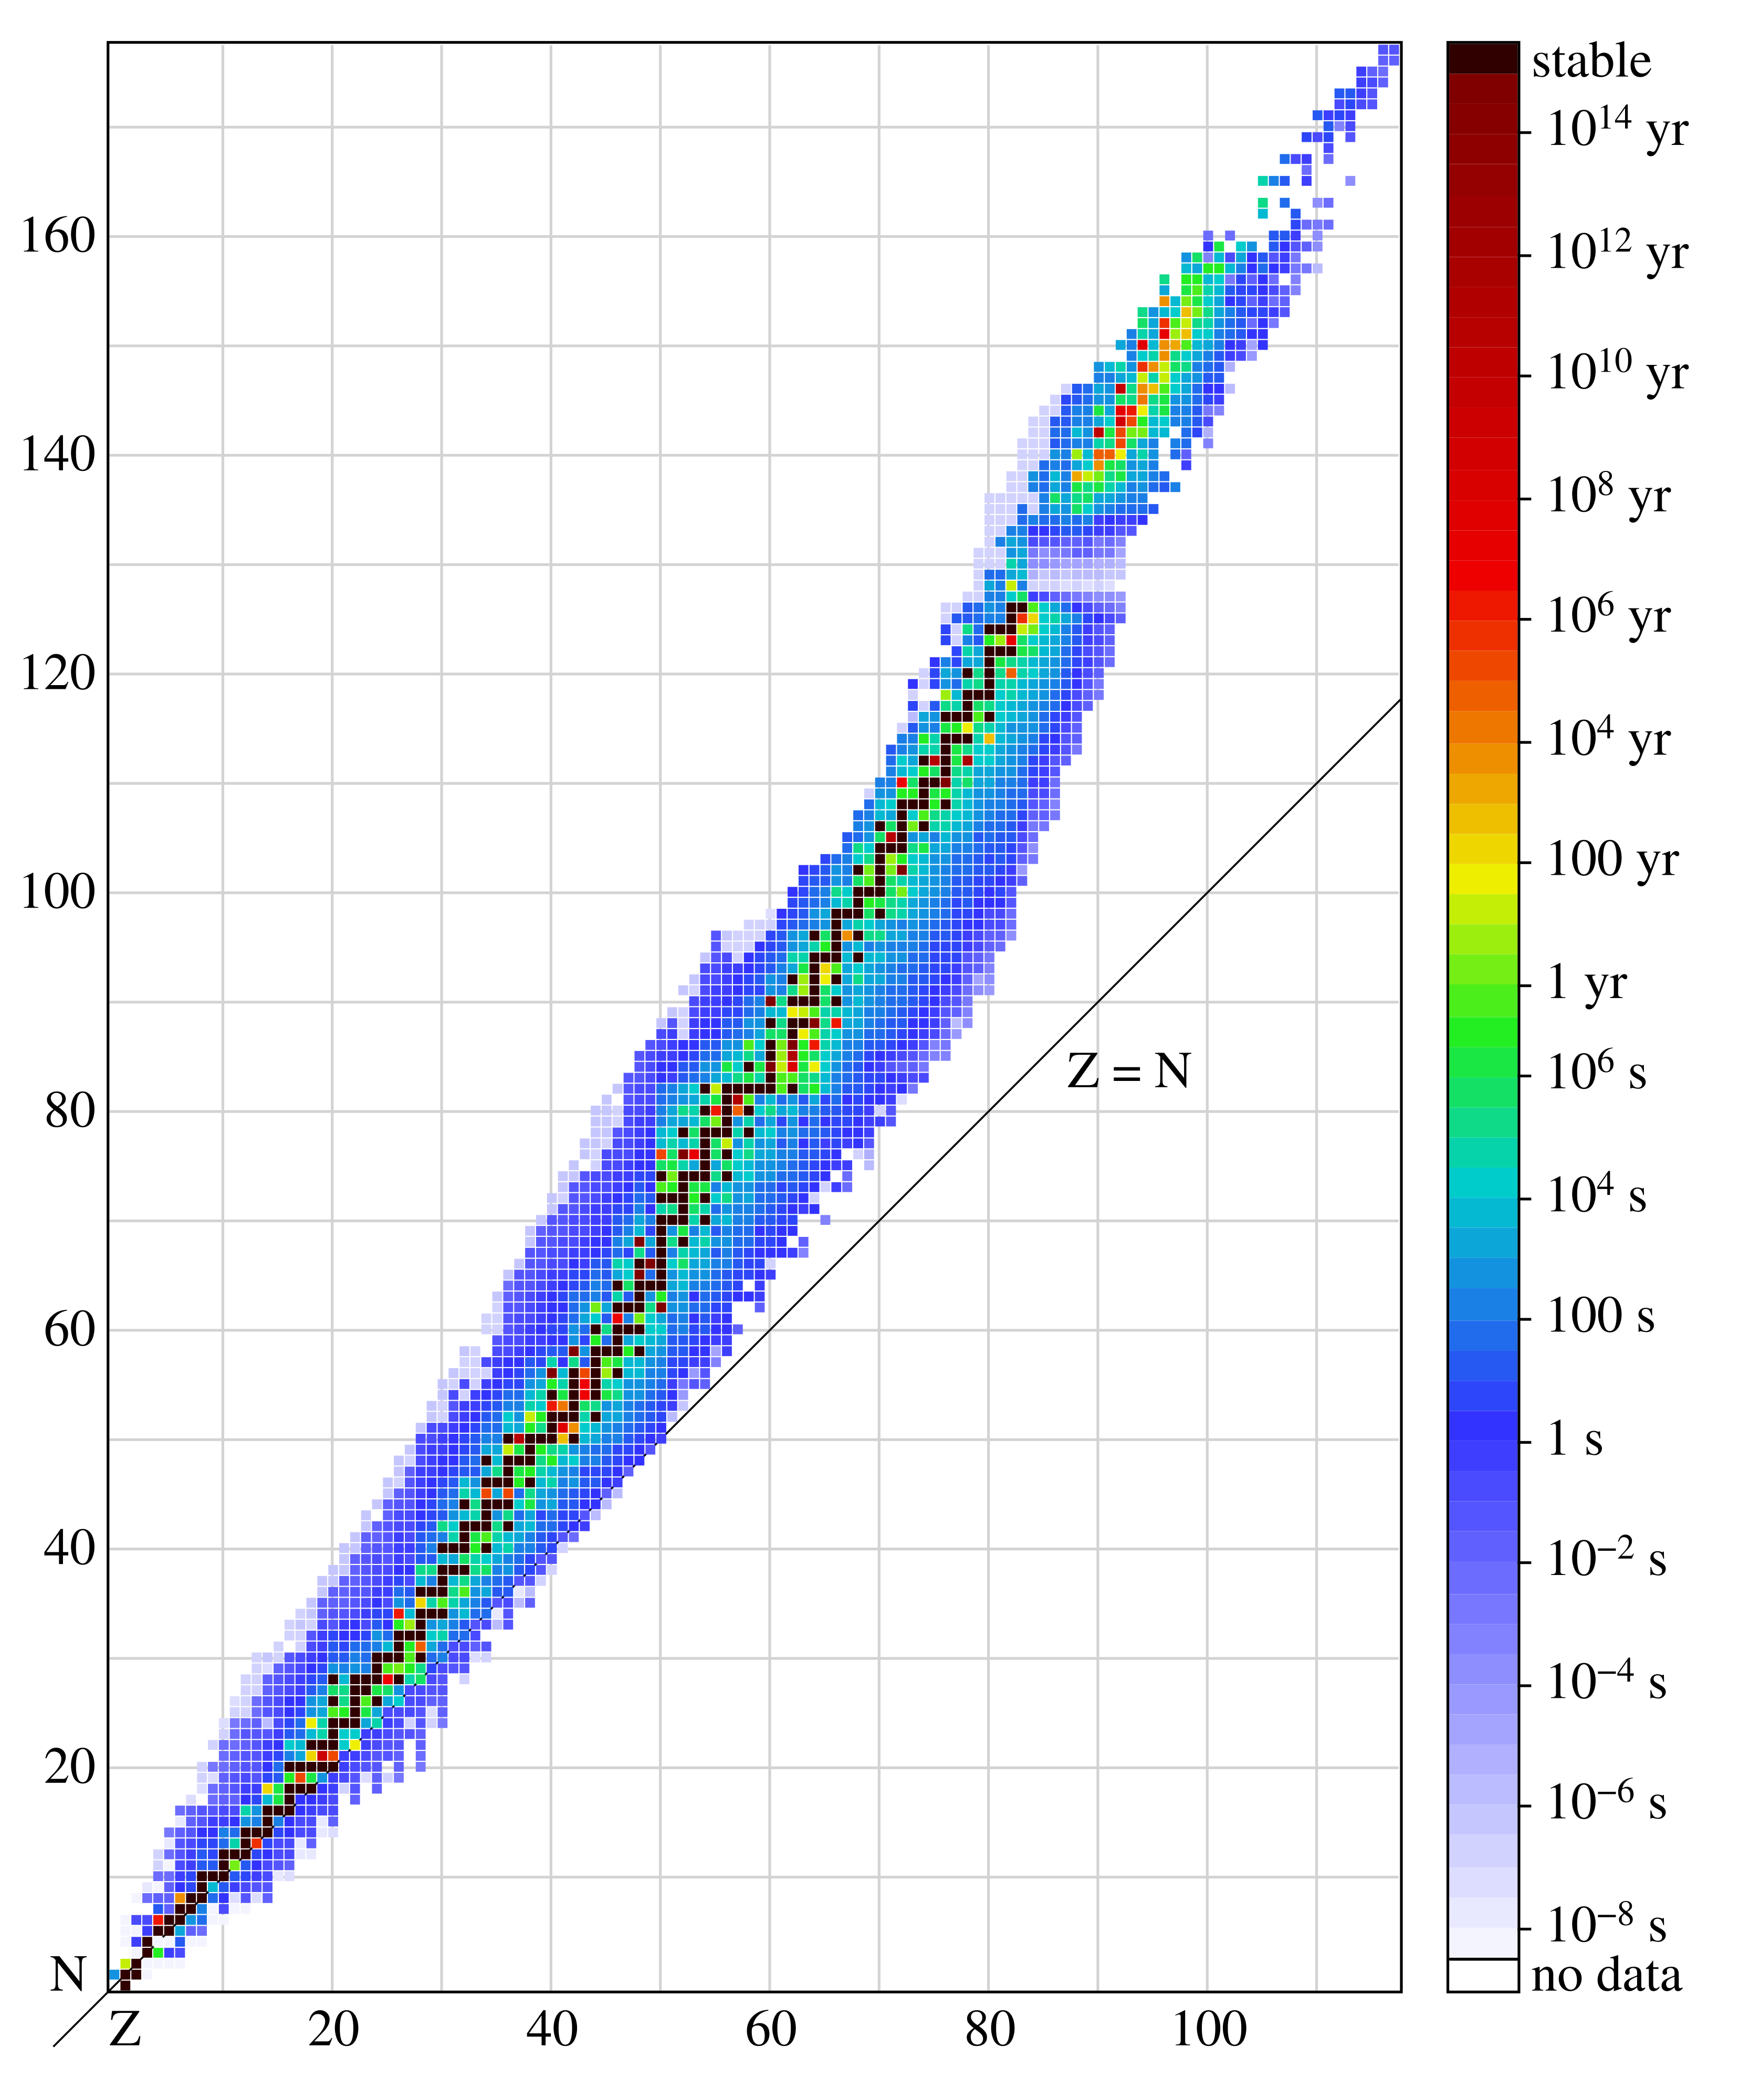
\includegraphics[height=12cm]{images/Isotopes_and_half-life.png}
\caption[Plot of neutron number against proton number for nuclei with half-lives greater than 10${^{-8}}$ s.]{Plot of neutron number against proton number for nuclei with half-lives greater than 10${^{-8}}$ s. Taken from \cite{BenRG}.}
\label{figure:NZcurve}
\end{figure}

Another characteristic feature of fission products is that their masses are bi-modally distributed. Figure \ref{figure:fissionyield} shows calculated fission yields as a function of mass number, indicating a 40:60 rather than 50:50 mass distribution among child nuclei when heavy nuclei are fissioned. This is attributed to smaller nuclei (which have high binding energies per nucleon) separating from the nucleus first at the moment when fission occurs. This results in the majority of fission products centering around atomic masses of 95 and 135, producing a disproportionate number of nuclei such as Sr, Y and Zr on the low side and Te, I and Cs on the high side of the distribution. 


% Iodine 0.1142684237, Tellurium 0.180582

\begin{figure}[ht]
\centering
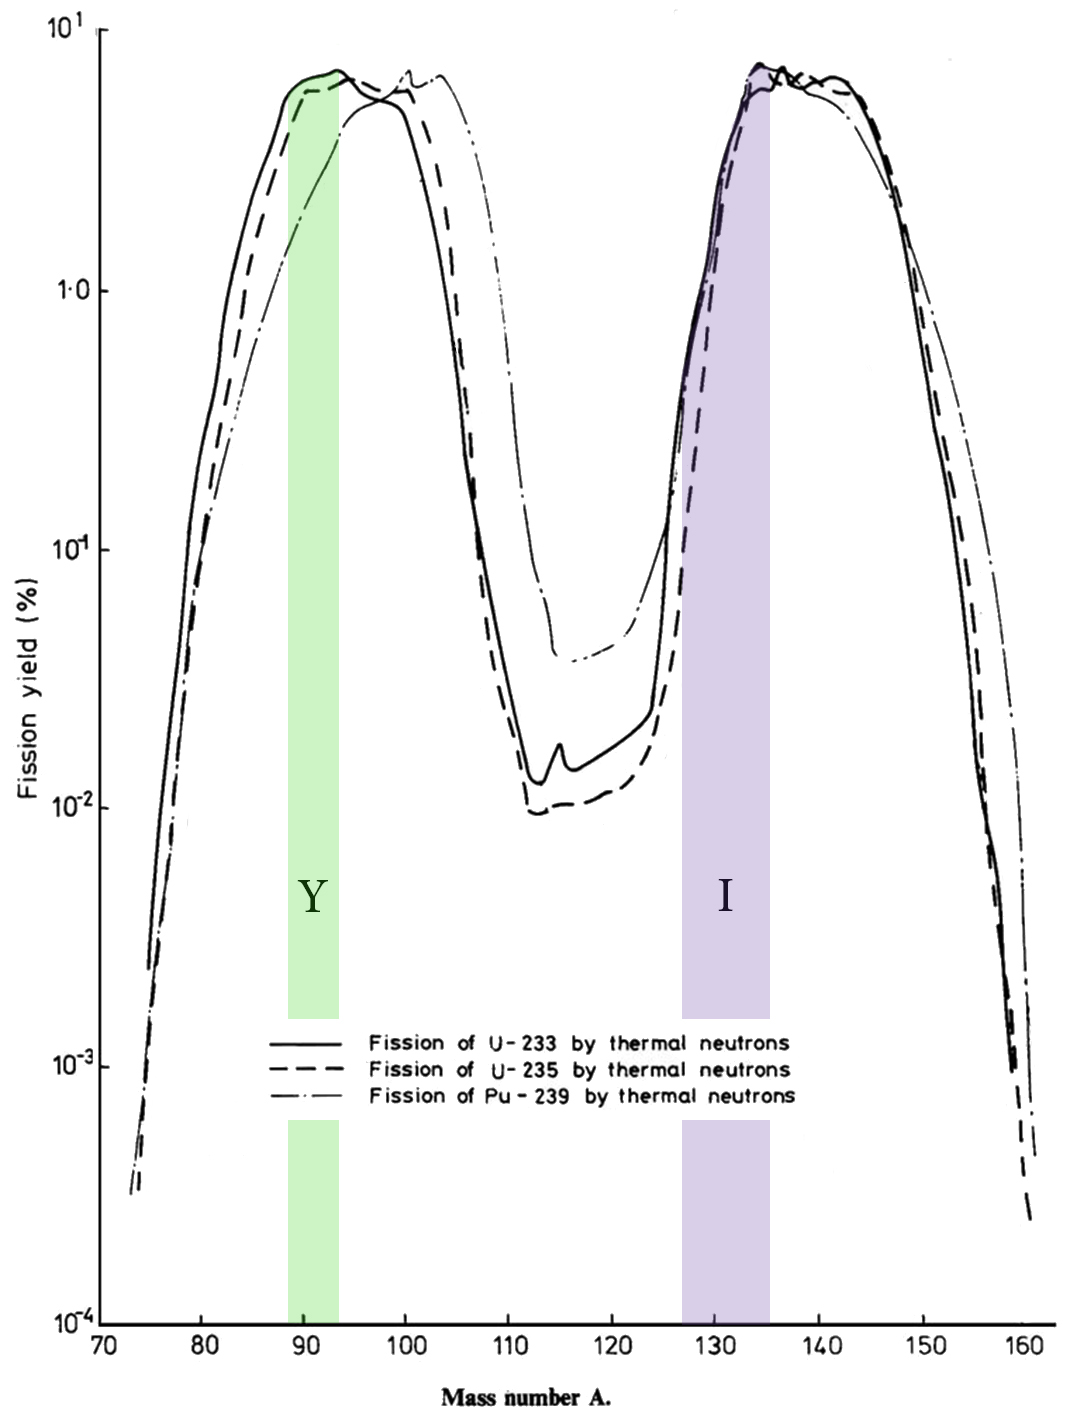
\includegraphics[height=12cm]{images/fissionyield.jpg}
\caption[Plot of the percentage yield of nuclei with a given mass following a fission event. Range of masses corresponding to isotopes of iodine shown in purple and isotopes of yttrium shown in green, based on Equation \ref{eqn:fission}.]{Plot of the percentage yield of nuclei with a given mass following a fission event. Range of masses corresponding to isotopes of iodine shown in purple and isotopes of yttrium shown in green, based on Equation \ref{eqn:fission}. Adapted from \cite{England1992}.}
% M. F. James, R. W. Mills and D. R. Weaver (1991) UKAEA Reports, AEA-TRS-1015, AEA-TRS-1018 
         %  and AEA-TRS-1019.
\label{figure:fissionyield}
\end{figure}

Iodine is an important fission product because it is known to corrode Zr metal cladding. It is part of the Te $\rightarrow$ Cs decay chain, with most isotopes exhibiting half-lives ranging from a few seconds to several days. Select data on Te and I fission yields are presented in Table \ref{table:decaydata_chap1}. In total, the independent yield of I isotopes from U$^{235}$ fission is 11.4\%, while the independent yield of Te isotopes (I precursors) is 18.1\%, with \ch{Te_{52}^{134}} having the highest independent yield of all possible fission products (6.3\%). These particular elements will also usually be paired with Zr and Y fission products, the latter of which is a common phase stabiliser dopant in \zirconia .

\begin{table}[ht]
\onehalfspacing
\caption{Independent fission product yields and half-lives for the major iodine isotopes and precursors in a thermal neutron reactor. Yields from the Joint Evaluated Fission and Fusion File (JEFF 3.3). All isotopes undergo single $\beta$- decay. Metastable states are included.}  \label{table:decaydata_chap1}
\begin{center}
\begin{tabular}{c c c}
\hline
Isotope & Independent Yield (\%) & Half-life \\
\hline
\texorpdfstring{I\textsubscript{131}}{I131} & 0.0029604
 & 8.023 d \cite{I131halflife} \\
\texorpdfstring{Te\textsubscript{132}}{Te132} & 1.5042 & 3.180 d \cite{Te132} \\
\texorpdfstring{I\textsubscript{132}}{I132} & 0.028399  & 2.295 h \cite{Te132} \\
\texorpdfstring{Te\textsubscript{133}}{Te133} & 3.9386 & 12.5 m \cite{khazov2011nuclear} \\
\texorpdfstring{I\textsubscript{133}}{I133} & 0.198194  & 20.87 h \cite{I133} \\
\texorpdfstring{Te\textsubscript{134}}{Te134} & 6.3001 & 41.8 m \cite{Sonzogni2004} \\
\texorpdfstring{I\textsubscript{134}}{I134} & 0.7673 & 52.5 m \cite{Sonzogni2004} \\
\texorpdfstring{Te\textsubscript{135}}{Te135} & 3.4777 & 19.0 s \cite{tellurium135halflife} \\
\texorpdfstring{I\textsubscript{135}}{I135} & 2.4635 & 6.58 h \cite{tellurium135halflife} \\ 
\texorpdfstring{Te\textsubscript{136}}{Te136} & 1.6652 & 17.63  s \cite{Mccutchan2018} \\
\texorpdfstring{I\textsubscript{136}}{I136} & 3.03823 & 83.4 s \cite{Mccutchan2018} \\
\texorpdfstring{Te\textsubscript{137}}{Te137} & 0.48440 & 2.49 s \cite{browne2007nuclear} \\
\texorpdfstring{I\textsubscript{137}}{I137} & 2.7026 & 24.5 s \cite{browne2007nuclear} \\ 
\texorpdfstring{Te\textsubscript{138}}{Te138} & 0.11280 & 1.4 s \cite{chen2017nuclear} \\ 
\texorpdfstring{I\textsubscript{138}}{I138} & 1.2419 & 6.26 s \cite{chen2017nuclear} \\  \hline
\end{tabular}
\end{center}
\end{table}

\section{Pellet-cladding interaction (PCI)}

At the beginning of a fuel pin's life, there is a gap between the fuel pellet and the cladding (see \ref{ss_fuelpin}). This gas gap slowly closes over time, mostly due to thermal expansion and swelling of the fuel pellet (illustrated in Figure \ref{figure:pcmi}) due to radiation damage. At a high enough burnup, the fuel pellet finally makes contact with the cladding. This phenomenon is called pellet-cladding interaction (PCI) and involves both mechanical and chemical interactions which contribute to observed fuel failures.

\begin{figure}[htp]
\centering
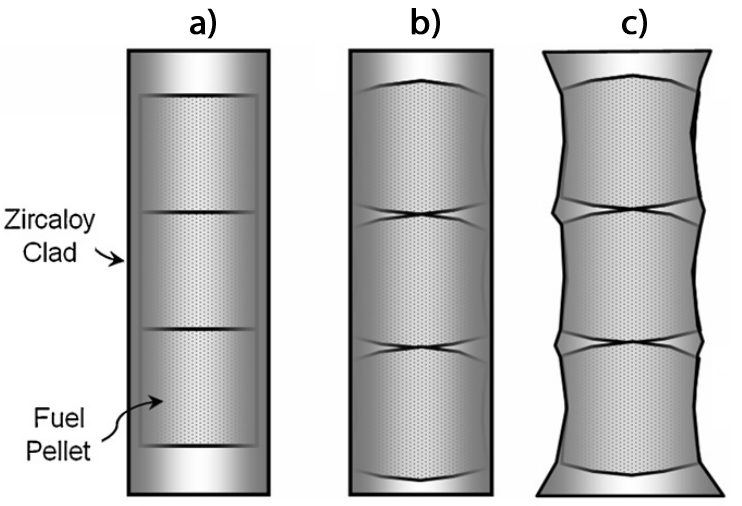
\includegraphics[height=9cm]{images/pcmi.png}
\caption[Illustration of fuel swelling and clad deformation due to PCI.]{Illustration of fuel swelling and clad deformation due to PCI. Adapted from \cite{alam2011review}.}
% M. F. James, R. W. Mills and D. R. Weaver (1991) UKAEA Reports, AEA-TRS-1015, AEA-TRS-1018 
         %  and AEA-TRS-1019.
\label{figure:pcmi}
\end{figure}

PCI-related failure of nuclear fuel pins has been known about since 1963, when the first reported failure occurred in a highly rated fuel pin during reactor start-up \cite{lyons1963high}. Many studies and reviews have since been made on the topic \cite{alam2011review, bcoxpelletclad1990}. The exact cause of PCI failures has not yet been discovered, however it is likely that both the mechanical and chemical effects of contact between the fuel pellet and the cladding are necessary. It is also known that PCI failures are typically preceded by power transients, such as during reactor startup where several power ramps are performed over many hours.

\subsection{Pellet-clad gap and bonding}

The gap between the fuel and the cladding allows fuel pellets to be inserted into the fuel pin easily during manufacture, but this clearance is also designed to accommodate some increase in fuel pellet volume. It is important to consider the thermal expansion of the fuel pellet, as the centreline temperature of a PWR fuel pellet during a power transient can vary between 1500 and 1800 $^{\circ}$C, depending on the burnup of the fuel and magnitude of the reactivity insertion \cite{Bagger1994}. In addition, fuel pellets will swell due to radiation damage throughout their operational lifetime. Once the pellet-clad gap has closed entirely, any pellet expansion during a power transient will translate to a force exerted on the cladding, generating hoop stresses which open cracks on the inner cladding surface. This is the mechanical component of PCI.

When the fuel pellet makes contact with the cladding, there is also a chemical interaction between the UO$_{2}$ (and fission products) and the internal surface oxide of the cladding. UO$_{2}$ has some solubility in ZrO$_{2}$, and we therefore see a bonded reaction layer which is of the form (U, Zr)O$_{2}$.  Due to the large U atom, cation substitution allows this layer to adopt the crystal structure of cubic fluorite, the high temperature phase of ZrO$_{2}$.

\subsection{Reactor power ramps}

It has been firmly established that PCI failures are associated with power ramping of the reactor. This presents a problem for reactors when it comes events such as start-up, load-following and any other power transients experienced by the fuel pins. Figure \ref{figure:reactor_startup} shows how reactor power varies over time during a typical PWR start-up procedure. A combination of low ramping rates and long holds at low power (to remain below ramping limits, condition fuel, and conduct coolant chemistry checks) require the entire procedure to be completed in a period of 90 hours, with several operator switch-overs in between. This is a costly procedure for the reactor operator to perform, with up to millions of US\$ foregone in electricity sales for bigger reactors, of which there are typically two or more per power plant. 

\begin{figure}[htp]
\centering
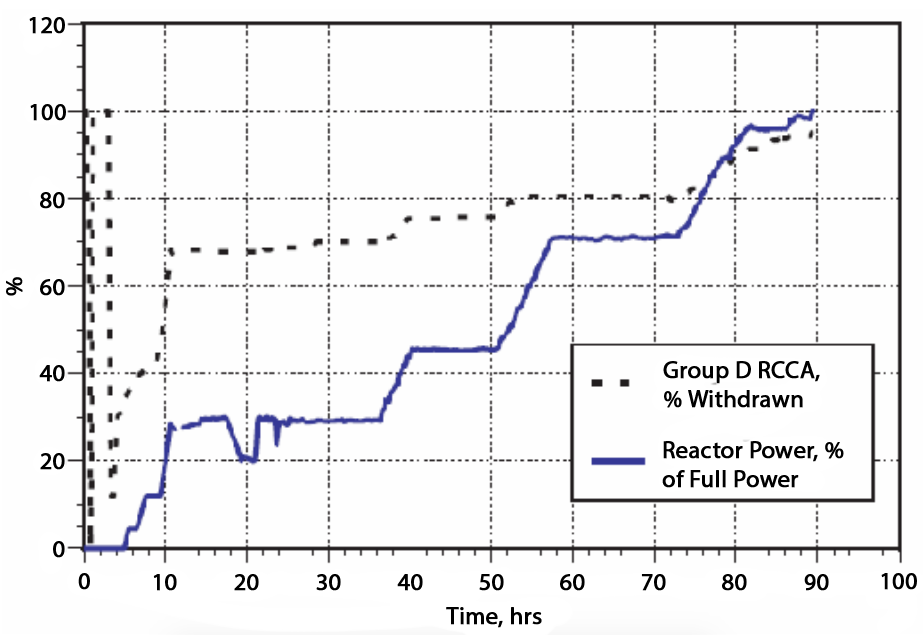
\includegraphics[height=10cm]{images/reactor_startup.png}
\caption[Reactor startup procedure for a typical US PWR. Dashed line indicates \% withdrawal of control rods.]{Reactor startup procedure for a typical US PWR. Dashed line indicates \% withdrawal of control rods. Adapted from \cite{ramping}.}
% M. F. James, R. W. Mills and D. R. Weaver (1991) UKAEA Reports, AEA-TRS-1015, AEA-TRS-1018 
         %  and AEA-TRS-1019.
\label{figure:reactor_startup}
\end{figure}

Scheduled reactor shutdowns or extended low power operation (ELPO) events occur whenever refuelling or maintenance of the reactor is required. Refuelling is typically performed every 1 to 2 years, while maintenance may be required at any time. Emergency shutdowns may also occur and have their own challenges to consider (e.g. xenon poisoning, decay heat removal), though they are more rare. In each case, going through the lengthy power ramping procedure is required, and since these shutdowns cannot be avoided, being able to ramp up power faster would be a significant improvement. Ramp rates in reactors are restricted to between 3-4\% of full power above a certain threshold level to avoid PCI failures \cite{ramping}. Additionally, fuel conditioning holds (operation at certain power levels for long periods) are performed to further reduce the incidence of PCI failures. 

These limits present a challenge not just when restarting reactors, but also for the implementation of load-following in reactors. Nuclear reactors have thermal feedback loops which provide some level of intrinsic load-following behaviour. For example, an increase in steam demand leads to increased boiling in the steam generators. The subsequent decrease in temperature of coolant leaving the steam generator causes a reactivity increase and therefore a power increase in the reactor. The reactor returns to critical (reactivity = 0) after some fluctuation, and the average temperature of the coolant remains unchanged.





\subsection{Iodine corrosion of zirconium}

B.Cox PCI failures of Zr alloy fuel cladding \cite{bcoxpelletclad1990} talks about how they found out that fission products were necessary for PCI failures on page 260 (citation 54)


\begin{figure}[htp]
\centering
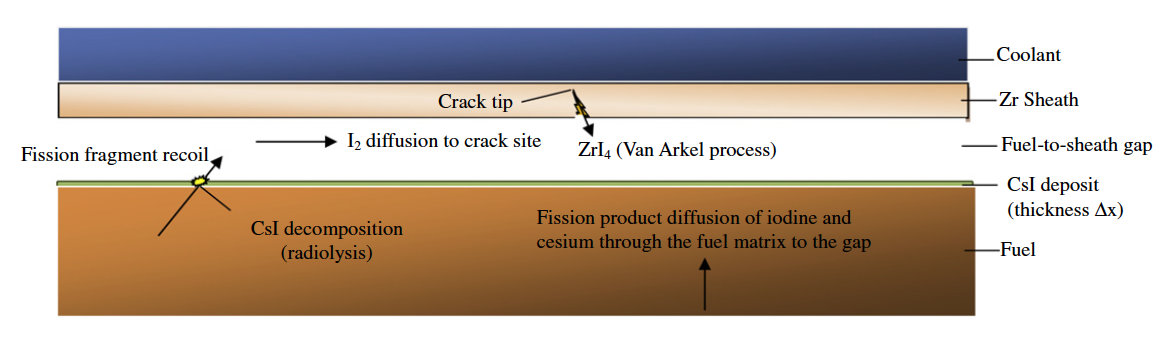
\includegraphics[width=16cm]{images/vanarkel.png}
\caption[Schematic of a proposed I-SCC process for cladding crack penetration.]{Schematic of a proposed I-SCC process for cladding crack penetration. Taken from \cite{Lewis2011}.}
\label{figure:vanarkel}
\end{figure}

\section{Oxidation of zirconium}

The oxidation of zirconium to produce \zirconia\ occurs during manufacture of the fuel cladding when the Zr metal is exposed to oxygen in air. \zirconia\ is a ceramic with material properties that make it desirable in many industrial applications, including solid-oxide fuel cells \cite{radford1979zirconia}, refractory linings \cite{whittemore1952fused}, and nuclear waste storage \cite{wang2012ceramics}. However, in the context of nuclear fuel cladding, the most important function of \zirconia\ is the barrier it provides to the ingress of corrosive species. 


\subsection{Oxide growth mechanism}

An oxide layer will typically form on the surface of zirconium metal even at very low oxygen partial pressures \cite{causey2005review}. The oxidation process is mainly driven by the ingress of oxygen ions. Initially, the oxide is highly protective, growing slowly into the metal until it reaches a thickness of approximately 2-3 $\mu$m \cite{garzarolli1991oxide,dawson1968kinetics}, after which the oxide growth mechanism enters a `post-transition' stage where the oxidation kinetics follow a cubic-rate law  \cite{porte1960oxidation}. At low temperatures relative to the melting point or high pressures, and after reaching a critical thickness (called the transition point), parts of the initial oxide will fail and the oxidation process will increase again. This process is illustrated in Figure \ref{figure:oxide_weight_gain}. 

\begin{figure}[htp]
\centering
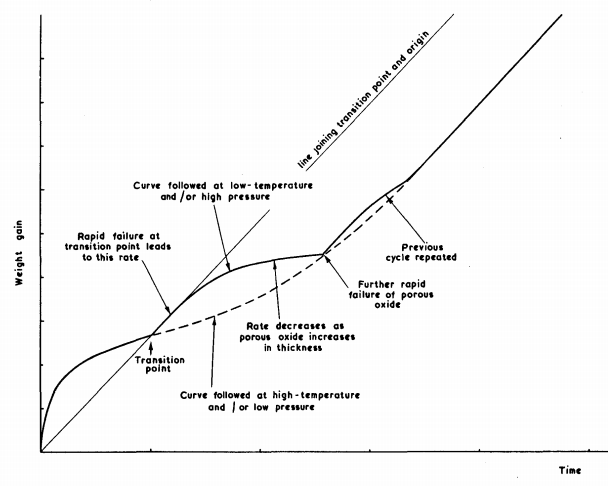
\includegraphics[height=10.5cm]{images/zro2_oxide_weight_gain.png}
\caption[Diagrammatic representation of the cyclical oxidation behaviour of \zirconia .]{Diagrammatic representation of the cyclical oxidation behaviour of \zirconia . Taken from \cite{cox1963some}.}
\label{figure:oxide_weight_gain}
\end{figure}

\subsection{Oxygen solubility of zirconium}

Looking at the Zr-O binary phase diagram in Figure \ref{figure:binary_phase_diagram}, oxygen is soluble in zirconium up to 29\% of total molar mass when below 400 $^{\circ}$C, the operating temperature region of a typical PWR. Solubility increases slightly up to 35\% of total molar mass as temperature is increased to the liquidus line at 2065 $^{\circ}$C. This is important to note because in the literature, studies often assume that there is pure Zr metal immediately beneath the \zirconia\ layer \cite{rossi2015first}, which is an assumption that will underestimate the extent to which repassivation occurs when the oxide layer is breached, and disregards the effect of the thin ZrO interface preceding the metal. The molar mass of oxygen required to grow more oxide near the interface will therefore be at least 37\% lower than expected when using this assumption.

The presence of oxygen in the Zr metal will also have an effect on thermodynamic calculations of extrinsic defect formation. Atoms such as Te and I will have to compete with O atoms (and to some extent, self-interstitial Zr atoms) for interstitial sites in the metal. This increases the energy barrier to diffusion because of the lower availability of sites. An energy input is required to remove O or Zr atoms occupying these sites, making them a less favourable diffusion path.


\begin{figure}[htp]
\centering
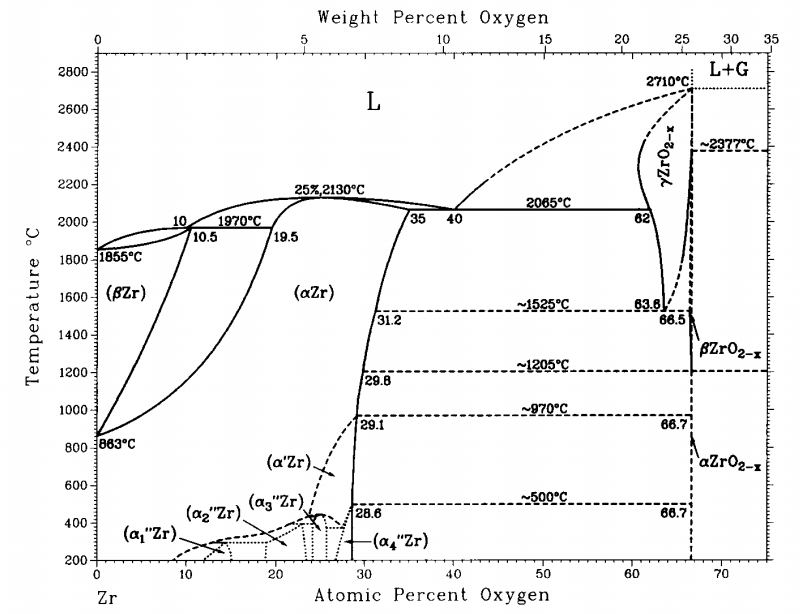
\includegraphics[width=14cm]{images/zro2_binary_phase.png}
\caption[Binary phase diagram of the Zr and O$_{2}$ system.]{Binary phase diagram of the Zr and O$_{2}$ system. Taken from \cite{Abriata1986}.}
\label{figure:binary_phase_diagram}
\end{figure}

\subsection{Outer oxide vs inner oxide}

As mentioned previously, the cladding of an LWR fuel pin develops an oxide on both the inner and outer surfaces due to exposure to oxygen in air during manufacture. Both the outer and inner oxide layers provide protection against corrosion, though the corrosive environment is different. 

The outer oxide layer is in contact with the coolant which is mostly light water with some additional dissolved species such as boron and hydrogen to control reactivity and pH. Figure \ref{figure:outer_oxide} shows a section of the cladding with the outer oxide visible. This layer is mostly monoclinic \zirconia\ with small grains of tetragonal \zirconia\ distributed uniformly throughout. These grains of tetragonal \zirconia\ are autostabilised during growth of the oxide because of the large volume expansion associated with oxidation (Zr has a Pilling-Bedworth ratio of 1.57). Of course, samples under examination are always stress-relieved, whereas cladding in reactor conditions will be under external hydrostatic pressure conditions (approximately 15 MPa), as well as internal pressure from fill gas and gaseous/volatile fission products.

\begin{figure}[htp]
\centering
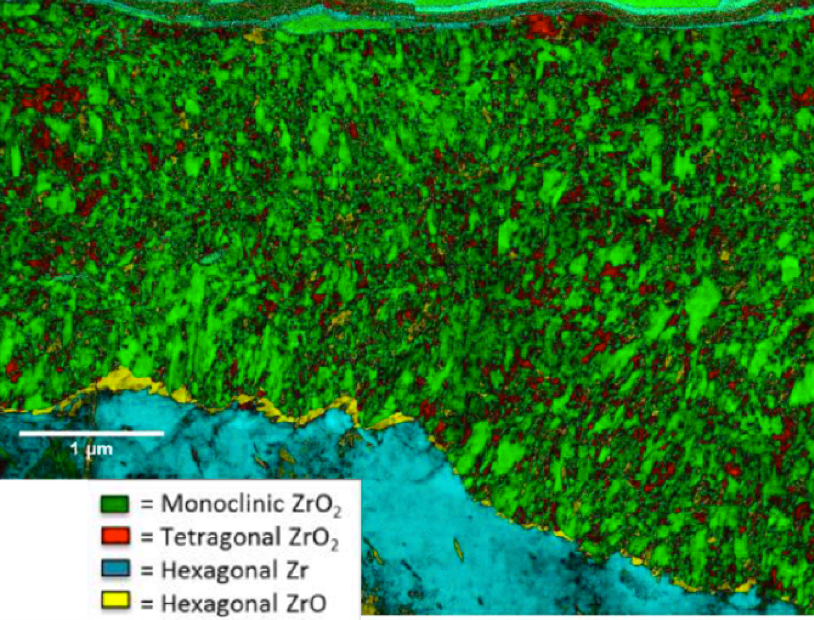
\includegraphics[height=10.5cm]{images/outer_oxide.png}
\caption[STEM image of the outer oxide layer showing the prevalence of different \zirconia\ phases.]{STEM image of the outer oxide layer showing the prevalence of different \zirconia\ phases.. Taken from \cite{Hu2016}.}
\label{figure:outer_oxide}
\end{figure}

The internal oxide layer is more challenging to examine. This layer is typically very brittle due to radiation damage and implantation of fission products. At a high enough burnup, the \zirconia\ layer makes contact with the UO$_{2}$ fuel and will also bond together. Figure \ref{figure:inner_oxide} shows a section of the cladding with the inner oxide layer bonded to the pellet. The crystal structure of the \zirconia\ in this layer is debated. Some studies report no monoclinic phase in high burnup fuels, with cubic phase \zirconia\ throughout most of the layer and an amorphous phase nearer the pellet side \cite{Nogita1997}, while other studies report mostly tetragonal phase in this layer. 
%After removal from the reactor and the subsequent cooling period, the inner oxide

\begin{figure}[htp]
\centering
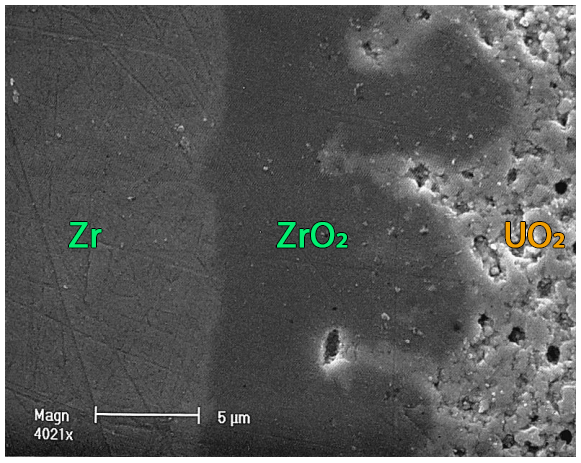
\includegraphics[height=10.5cm]{images/pci_bondinglayer.png}
\caption[High resolution SEM image of the bonding layer between a PWR UO$_{2}$ fuel pellet and Zr cladding in a fuel pin at an approximate burnup of 60 GWd/tU.]{High resolution SEM image of the bonding layer between a PWR UO$_{2}$ fuel pellet and Zr cladding in a fuel pin at an approximate burnup of 60 GWd/tU. Taken from \cite{Lozano1998}.}
\label{figure:inner_oxide}
\end{figure}

Figure \ref{figure:bonding_layer_composition} shows the composition of the inner oxide of a high burnup fuel pin. The fission product (Ba, Mo, Nd) content is highest at the beginning of the \zirconia\ layer and decreases almost linearly with distance towards the Zr metal. This is due to fission product implantation rather than diffusion as these are highly immobile atoms. % can you use the weight composition and fission yields to estimate what percentage of iodine implantation will be?

\begin{figure}[htp]
\centering
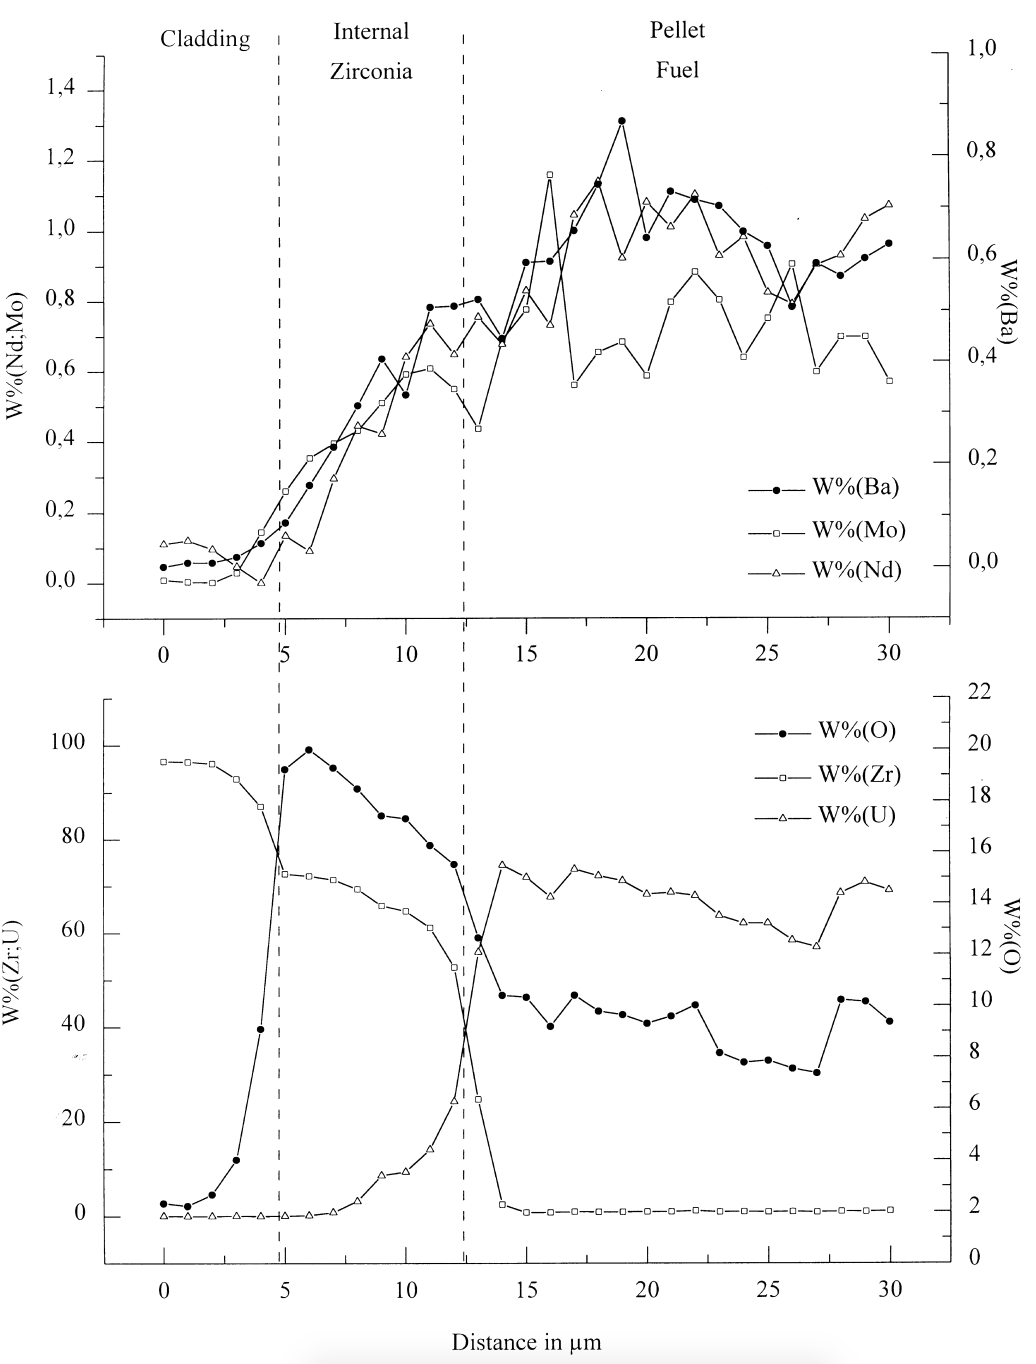
\includegraphics[width=14cm]{images/bonding_layer_composition.png}
\caption[Elemental composition of the bonded UO$_{2}$/ZrO$_{2}$ layer.]{Elemental composition of the bonded UO$_{2}$/ZrO$_{2}$ layer. Taken from \cite{Lozano1998}.}
\label{figure:bonding_layer_composition}
\end{figure}



\subsection{Sources of oxygen}

The internal oxide layer is present before fuel claddings are pressurised with helium gas and sealed. This is from the normal oxidation of Zr in air, where the oxygen pressure is 0.21 atm. After capping of the fuel rods, the only other available oxygen is from the UO$_{2}$ fuel pellets.

Uranium oxides have a wide range of non-stoichiometric compositions, with U/O ratios ranging from 1.67 to 2.24 in solid UO$_{2 \pm x}$, as shown in Figure \ref{figure:U_O_phase_diagram}. The oxide form U$_{3}$O$_{8-y}$ also exists and is more kinetically and thermodynamically stable than UO$_{2}$, but has lower density, making it less suitable for use as a fuel form. The different stoichiometries have different equilibrium O$_{2}$ pressures at constant temperature, allowing some level of tweaking the internal cladding environment depending on whether more or less oxygen is desired. 

Oxygen and oxygen precursors may also be produced directly from fission of U
$_{235}$, but this contribution is insignificant compared to changing the stoichiometry of the fuel pellet. Indeed, liberation of oxygen from UO
$_{2 \pm x}$ due to fission (which is also a function of the fuel's stoichiometry) is a more significant contributor to the oxygen pressure than direct production via fission.

\begin{figure}[htp]
\centering
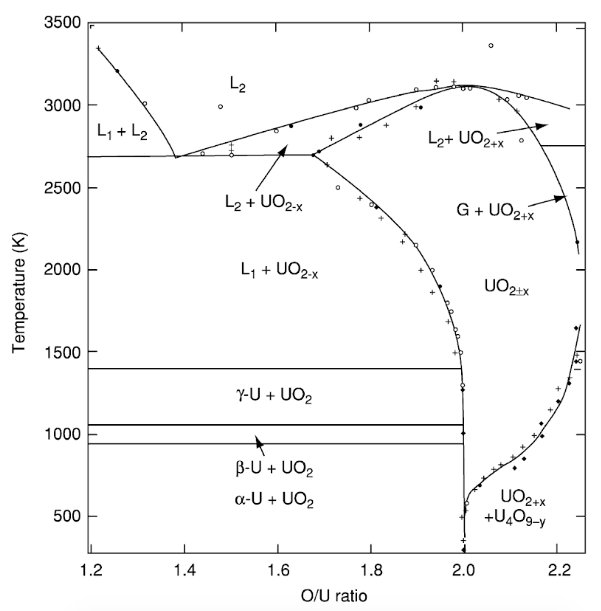
\includegraphics[height=12cm]{images/UO_phase_diagram.png}
\caption[Partial U-O temperature phase diagram between O/U ratios of 1.2 and 2.25.]{Partial U-O temperature phase diagram between O/U ratios of 1.2 and 2.25. Figure taken from \cite{katz2007chemistry}, with phase boundaries from \cite{rand1978thermodynamic, chevalier2002progress, gueneau2002thermodynamic}.}
\label{figure:U_O_phase_diagram}
\end{figure}


\section{Atomistic Simulation}

Conducting experiments on nuclear materials is a difficult undertaking. Nuclear grade materials are expensive (e.g. high purity zirconium), and materials such as uranium are highly controlled (though they are relatively benign compared to many typical chemical laboratory materials and solvents). Furthermore, experiments which require samples to be irradiated must be left to cool-down (due to material activation) for up to a year before they can be analysed in a specialised lab \cite{efthymiopoulos2011hiradmat}. This makes it difficult to study many material phenomena, especially if they are time-dependent. In-situ reactor experiments are also problematic, requiring sensor equipment to be ruggedised for high radiation environments as well as obtaining special permission from a reactor operator (and the paperwork that entails) to conduct  such a test. Any errors in the experimental procedure or problems with samples are not revealed until months later when material analysis is performed. The risks and costs make it such that experimental work is mostly restricted to the largest labs and the few researchers with enough funding to support it.



\subsection{Classical approach - molecular dynamics}

Molecular dynamics (MD) uses classical mechanics as the basis for calculations. These types of simulations typically use pair potentials (though many-bodied potentials are also used). These are mathematical functions which effectively describe the electronic interaction between two particles. Pair potentials are created by fitting functions to several parameters from empirical data, such as equilibrium bond lengths, thermal properties or even values from quantum mechanical calculations. The simple form of pair potentials allows MD simulations to scale up to billions of atoms, corresponding to a length scale of approximately 0.1 $\mu$m. 

In the literature, many molecular dynamics studies of \zirconia\ exist. However, these studies typically focus on dopant-stabilised zirconias. The large system sizes possible in molecular dynamics simulations are often necessary for examining properties such as ion diffusion, thermal conductivity or melting points \cite{Davis2010}. Studying fission products in \zirconia\ however, requires potentials which can accurately model atoms such as Zr, O, and I in the solid phase. A good potential for such a system has not yet been published and so a quantum mechanical study of the \zirconia\ system is the focus of this thesis. The work herein may then be used in the future development of such potentials.

%These relatively large system sizes make MD a useful tool for studying a range of materials phenomena which are difficult to model at smaller scales, such as dislocations and long-range diffusion. 

%Add a figure here showing lennard jones. Also show the basic equations
%These are mainly pair potentials (although many-bodied potentials are also used) which are some combination of a short-range repulsion term (Pauli exclusion, nuclear repulsion if van der waals is taken into account) and a long range Coulombic attraction term

\subsection{Quantum mechanical approach - DFT}

Another method for modelling materials at the atomic scale is to use a quantum mechanical approach. In this thesis, the framework of density functional theory (DFT) is used throughout for quantum mechanical calculations (see § \ref{section:dft}). These techniques use a more fundamental approach than molecular dynamics, and are sometimes referred to as \emph{ab initio} methods (though several empirical approximations are often used in DFT).  

System sizes are far more constrained when using DFT. The equations being solved scale combinatorially with the number of electrons and ions in the system, quickly becoming intractable even for simple molecules with a few atoms. However, there are several ways to significantly reduce the computational complexity without sacrificing too much accuracy (e.g. the pseudopotential method, periodic boundaries, cell constraints and symmetry). This allows system sizes on the order of hundreds of atoms to be studied, corresponding to a length scale of approximately 1 nm. While this length scale is much smaller than what can be achieved using MD, the use of a more fundamental parameter (electron density) in calculations provides a stronger scientific basis when material properties are derived from DFT models. Additionally, DFT allows electronic properties such as electron orbital occupancy and band gaps to be studied.

\subsection{Band gap}

Materials are generally considered to fall into one of two categories; conductors or insulators. While this binary characterisation may work as an approximation for many materials, in reality there is more of a continuum between these two states, and at the heart of this lies the band gap.

It is known that for ions, electron energy levels are quantised, restricting the range of possible electron energies to discrete quantities. More specifically, electrons can only occupy unique quantum states, defined by parameters such as quantum spin and angular momentum. In a crystal, where there are large numbers of electrons and many possible configurations of them, we refer to energy "bands" which are comprised of many quantised energies. There are sometimes gaps between energy bands in crystals (illustrated in Figure \ref{figure:band_gap}) corresponding to energy levels that cannot be occupied, meaning that if electrons were to be added at the lowest energy levels one by one, there would occasionally be relatively large jumps in energy as an electron is forced to enter a higher energy band. 

\begin{figure}[htp]
\centering
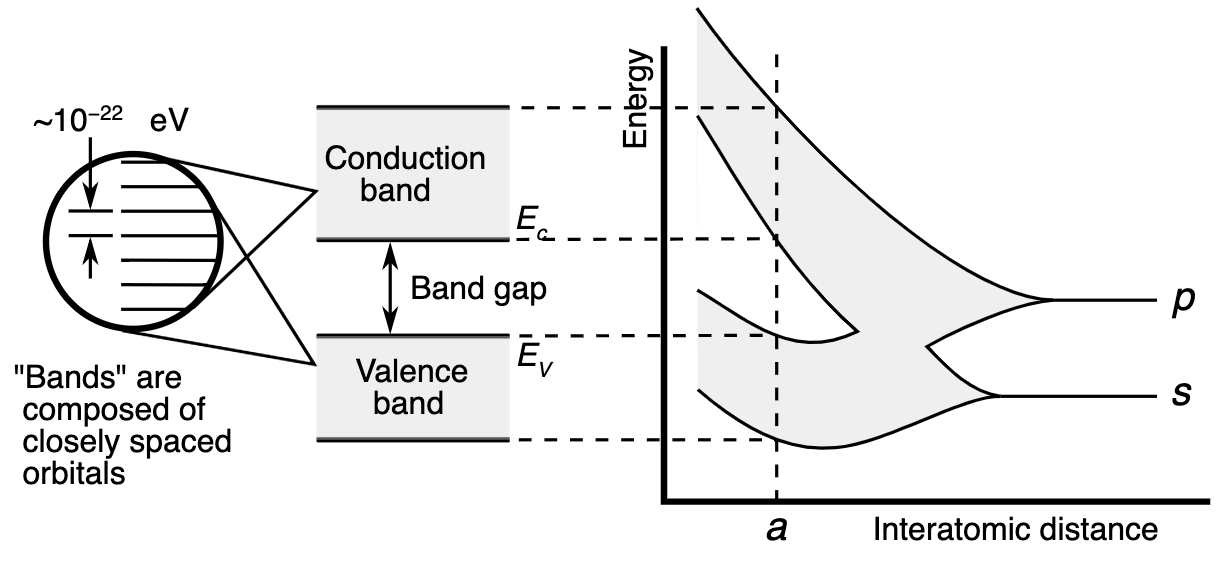
\includegraphics[width=\linewidth]{images/band_gap.png}
\caption[Illustration of the band gap in diamond as a function of interatomic spacing.]{Illustration of the band gap in diamond as a function of interatomic spacing. Taken from \cite{Chetvorno2017}.}
\label{figure:band_gap}
\end{figure}

Two energy bands, called the valence band and conduction band, help determine a material's metallic or non-metallic character. The valence band contains energy levels occupied by the valence electrons (at absolute zero), while the conduction band contains energy levels which are high enough that electrons may freely move throughout the crystal. In metals, the valence and conduction bands have some amount of overlap, meaning that once the valence band is full, the highest occupied electron energy states are within the conduction band and so the material acts as a conductor. Materials like \zirconia , however, have large energy gaps between the valence and conduction bands, known as the band gap. These materials are called "band insulators" (as opposed to Mott insulators), because the band gap is an energy barrier preventing the valence electrons from moving freely around the crystal.

In addition to the valence and conduction bands, we also need a value for the electron chemical potential or Fermi level of the material to determine how the energy bands are filled. If the Fermi level is exactly halfway between the valence band maximum (VBM) and the conduction band minimum (CBM), then the additional energy input required to promote an electron to the conduction band is half of the band gap. The Fermi level is strongly dependent on extrinsic defects and temperature. Extrinsic defects (called dopants) can be introduced to materials such as semiconductors in order to change the concentration of electronic defects (electrons and holes), while an increase in temperature will result in an increase in the Fermi level because of the larger amount of thermal energy available.

It is important to note that band gaps reported in DFT studies are significantly lower than those obtained experimentally. This is a known problem in DFT, and an exchange-correlation functional which reproduces correct band gap energies in semiconductors and insulators (without overfitting to experimental data) has not yet been discovered. In many cases, the band gap from DFT calculations may be increased by appending an additional potential term, known as a +U parameter, to certain valence electron orbitals. This is discussed further in § \ref{subsection:plus_U}.






